\newpage
\section{Architektura}
Nasza biblioteka składa się z wielu współpracujących ze sobą modułów:
\begin{figure}[!ht]
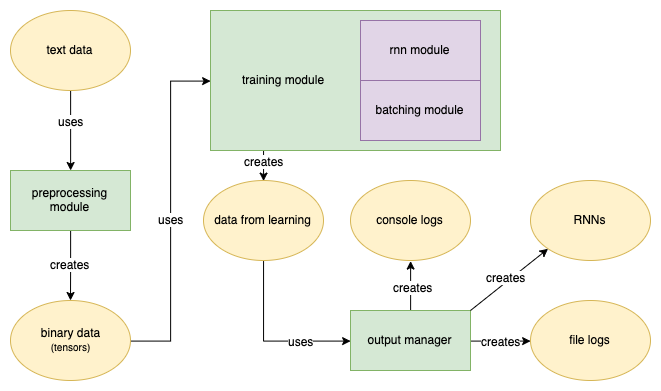
\includegraphics[width=\linewidth]{./images/modules.png}
\caption{schemat modułów biblioteki}
\label{fig:test3}
\end{figure}

\subsection{Moduł preprocesingu}
Największy i całkowicie niezależny od pozostałych części biblioteki moduł, którego zadaniem jest 
przetworzenie tekstów z formy tekstowej na formę binarną (tensory), która jest następnie wykorzystywana
do szkolenia sieci. Na tym etapie następuje również redukcja znaków w tekście, tak by wyeliminować
informacje, które nie są potrzebne z perspektywy szkolenia sieci. Teksty po przetworzeniu są 
zapisywane na dysku i mogą być wykorzystywane wielokrotnie. 
Wadą tego modułu jest długość przetwarzania tekstów, która trwa zwykle kilkanaście sekund oraz spora ilość
przestrzeni dyskowej i RAMu które są wykorzystywana w wyniku tego procesu.

\subsection{Moduł batchowania}
Moduł, który korzystając z dostarczonych danych binarnych dzieli je na batche i dostarcza modułowi treningowemu.
Pozwala na specyfikowanie parametrów tych danych, jak na przykład rozmiar batcha.
Decyduje również o tym kiedy kończy się proces uczenia oraz o losowości ustawienia autorów w batchu. 
Jego kod jest ściśle powiązany z kodem modułu treningu sieci ale z racji na obszerność zdecydowaliśmy 
się go wyodrębnić jako osobny moduł. 
Jest on niezależny od modułu preprocesingu, jednak format danych wyjściowych z modułu preprocesingu 
jest zbieżny z formatem danych wejściwych wymaganym przez modułu batchowania. 

\subsection{Moduł sieci} 
Moduł sieci jest małym modułem odpowiedzialnym za deklarację sieci neuronowej w PyTorchu.
 
\subsection{Moduł treningu sieci}
Ten moduł spina moduł sieci, oraz moduł batchowania przprowadzając za ich pomocą proces treningu sieci.
To w kodzie tego modułu następuje interacja przez epoki, przekazywanie danych z modułu batchowania 
do sieci, wykorzystanie funkcji kosztu, propagacja wsteczna i wszystkie inne składniki potrzebne do 
szkolenia sieci. 

\subsection{OutputManager}
Ten moduł odpowiedzialny jest za odbieranie danych z modułu treningu sieci, a następnie tworzenie z nich
wygodnego do analizy wyjścia. Wyjście to jest realizowane w formie danych ze szkolenia wyświetlanych 
w konsoli oraz zapisywanych do pliku csv, w formie parametrów sieci, które są zapisywane
w pliku txt oraz w formie kolejnych modeli sieci, które są zapisywane na dysku. 
Logi w konsoli pozowiły nam na wygodne kontrolowanie procesu szkolenia, dane w plikach csv potrzebne 
nam były do rysowania wykresów.

\newpage
\subsection{Skrypty - Prometheus}
\begin{enumerate}
	\item {\texttt{create\_scripts.py} } - 
	tworzy skrypty rozpoczynające uczenie sieci. Korzysta z pliku konfiguracyjnego \texttt{to\_run.json}.
	Zawartość pliku to run wraz z przykładowymi parametrami:
	
	\begin{import}
		[
		  {
		    "beginning": "#!/bin/sh",
		    "name": "#SBATCH -J test",
		    "node_numbers": "#SBATCH -N 1",
		    "tasks_per_node": "#SBATCH --ntasks-per-node=1",
		    "mem_per_cpu": "#SBATCH --mem-per-cpu=5GB",
		    "time": "#SBATCH --time=00:20:00",
		    "grant_name": "#SBATCH -A ap2018",
		    "partition": "#SBATCH -p plgrid",
		    "output": "#SBATCH --output=",
		    "errors": "#SBATCH --error=",
		    "hidden_size": "100",
		    "num_layers": "2",
		    "num_epochs": "5",
		    "batch_size": "40",
		    "timesteps": "50",
		    "learning_rate": "0.04",
		    "authors_size": "100",
		    "vocab_size": "48",
		    "save_path": "../results/",
		    "learning_tensors_path": "../data/dutch/tensors/known/",
		    "testing_tensors_path": "../data/dutch/tensors/known/",
		    "language": "DU"
		  }
		]
	\end{import}
	
	Poza standardowymi parametrami sieci opisanymi w podręczniku użytkowania występują również parametry
	związane z samym Prometheusem:
	\begin{itemize}
	  \item name - Nazwa zlecenia
	  \item node\_numbers - Liczba alokowanych węzłów
	  \item task\_per\_node - Liczba zadań per węzeł
	  \item mem\_per\_cpu - Ilość pamięci przypadającej na jeden rdzeń obliczeniowy
	  \item time - Maksymalny czas trwania zlecenia
	  \item grant\_name - Nazwa grantu do rozliczenia zużycia zasobów
	  \item partition - Specyfikacja partycji
	  \item output - Plik ze standardowym wyjściem
	  \item errors - Plik ze standardowym wyjściem błędów
	\end{itemize}
	
	Po wykonaniu komendy \texttt{python3 create\_scripts.py} w katalogu \texttt{scripts} zostaną 
	wygenerowane skrypty pozwalające na uczenie sieci z podanymi parametrami oraz tworzy foldery 
	wynikowe dla danej nazwy zlecenia.
	
	
	
	\item {\texttt{run.sh} } - 
	Uruchamia skrypty utworzone poprzez \texttt{create\_scripts.py} odpowiednio je kolejkując. Należy
	pamiętać o wcześniejszej inicjalizacji skryptów z parametrami opisanymi powyżej.
	
	\item {\texttt{copy\_data\_to\_prometheus.sh} } - 
	Pozwala na przesłanie plików. Wykorzystywany do przesyłania korpusu tekstów.
	
	\item {\texttt{draw\_plots.py} } -
	Przedstawia wyniki w formie wykresów.
	
	\item {\texttt{clean.sh} } -
	Czyści dotychczasowe wyniki.
	
	
	
\end{enumerate}



